\chapter{State of the Art}
\label{stateofart}
\thispagestyle{plain}

In this section, we review the state-of-the-art of the problem at hand. We start by describing why timetabling is a rather complex problem, some possible approaches to solve it and some of the existing solutions, specifically for the \gls{itc2007} benchmarks.\\

\section{Timetabling Problem}

When solving timetabling problems, it is possible to generate one of multiple types of solutions which are \textit{feasible}, \textit{non feasible}, \textit{optimal} or \textit{sub-optimal}. A feasible solution solves all the mandatory constraints, unlike non feasible solutions. An optimal solution is the best possible feasible solution given the problem constraints. A problem may have multiple optimal solutions. Lastly, non-optimal solutions are feasible solutions that have sub-optimal values.\\
\\
Timetabling automation is a subject that has been a target of research for about 50 years. The timetabling problem may be formulated as a search or an optimization problem~\cite{Schaerf1999}. As a search problem, the goal consists on finding a feasible solution that satisfies all the hard constraints, while ignoring the soft constraints. By posing the timetabling problem as an optimization problem, one seeks to minimize (considering a minimization problem) the violations of soft constraints while satisfying the hard constraints. Typically, the optimization is done after the use of a search procedure for finding an initial feasible solution.\\
\\
The basic examination timetabling problem, where only the \textit{clash} hard constraint is observed, reduces to the graph coloring problem~\cite{Jensen2001}, which is a well studied problem. The clash hard constraint specifies that no conflicting exams should be scheduled at the same time slot. Deciding whether a solution exists in the graph coloring problem, is a NP-complete problem~\cite{Arora2009}. Considering the graph coloring as an optimization problem, it is proven that the task of finding the optimal solution is also a NP-Hard problem \cite{Arora2009}. Graph Coloring problems are explained further in Section \ref{section:existingappr}
\\
%%%%%%%%%%%%%%%%%%%%
\section{Existing Approaches}
\label{section:existingappr}
%%%%%%%%%%%%%%%%%%%%
\begin{figure}[h!]
 \centering
   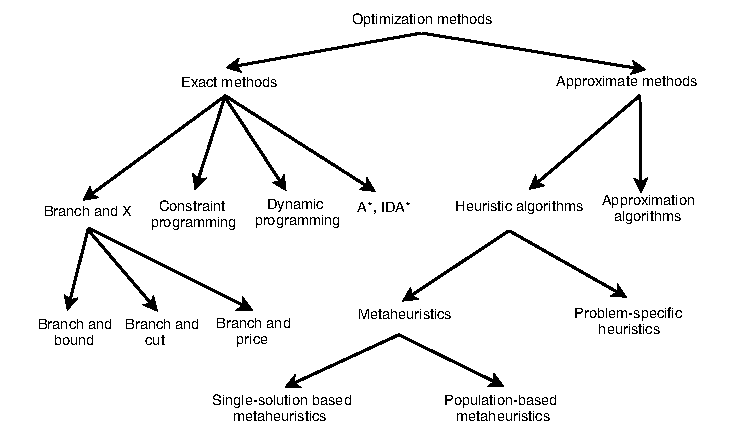
\includegraphics[width=1\textwidth,natwidth=1317,natheight=814]{./images/typesOfAlgorithms.pdf}
   \caption{Optimization methods: taxonomy and organization (adapted from \cite{Talbi2009}).}
   \label{fig:TypesAlgorithms}
\end{figure}

Figure~\ref{fig:TypesAlgorithms} depicts a taxonomy for the known optimization methods. These methods are divided into \textit{Exact methods} and \textit{Approximate methods}.\\
\\
Timetabling solution approaches are usually divided into the following categories~\cite{Qu2009}: \textit{exact algorithms} (Branch-and-Bound, Dynamic Programming), \textit{graph based sequential techniques}, \textit{local search based techniques} (Tabu Search, Simulated Annealing, Great Deluge), \textit{population based algorithms} (Evolutionary Algorithms, Memetic algorithms, Ant Colony algorithms, Artificial immune algorithms), \textit{Multi-criteria techniques}, \textit{Hyper-heuristics}, \textit{Decomposition/clustering techniques}. Hybrid algorithms, which combine features of several algorithms, comprise the state-of-the-art. Due to its complexity, approaching the examination timetabling problem using exact method approaches can only be done for small size instances. Real problem instances found in practice are usually of large size, making the use of exact methods impracticable. Heuristic solution algorithms have been usually employed to solve this problem.\\
\\
Real problem instances are usually solved by applying algorithms which use both \textit{heuristics} and \textit{meta-heuristics}. Heuristic algorithms are problem-dependent, meaning that these are adapted to a specific problem in which one can take advantage of its details. Heuristics are used to generate a feasible solution, focusing on solving all hard constraints only. Meta-heuristics, on the other hand, are problem-independent. These are used to, given the feasible solution obtained using heuristic algorithms, generate a better solution focusing on satisfying as many soft constraints as possible.\\
\\
Most of the existing meta-heuristic algorithms belong to one of the following three categories: One-Stage algorithms, Two-Stage algorithms and algorithms that allow relaxations~\cite{Lewis2007}. The One-Stage algorithm is used to get a solution, which the goal is to satisfy both hard and soft constraints at the same time. The Two-Stage algorithms are the most used types of approaches. This category is divided in two phases: the first phase consists in not considering the soft constraints and focusing on solving hard constraints to obtain a feasible solution; the second phase is an attempt to find the best solution, trying to solve the largest number of soft constraints as possible, given the solution of the first phase. Algorithms that allow relaxation can weaken some constraints in order to solve the \textit{relaxed problem}, while considering the elimination the used relaxations.

\subsection{Exact methods}
\label{subsection:exactmethods}
Approximation algorithms like heuristics and meta-heuristics proceed to enumerate partially the search space and, for that reason, they can't guarantee finding the optimal solution. Exact approaches perform a complete enumeration of the search space and thus guarantee that the encountered solution is optimal. A negative aspect is the time taken to find the solution. If the decision problem is very difficult (e.g. NP-Complete), in practical scenarios, given large size problem instances, using this approach may not be possible due to the long execution time.\\

\subsubsection{Constraint-Programming Based Technique}
The gls{cpbt} allows direct programming with constraints which gives ease and flexibility in solving problems like timetabling. Two important features about this technique are the use of backtracking and logical variables. Constraint programming is different from other types of programming, as in these types it is specified the steps that need to be executed, but in constraint programming only the properties (hard constraints) of the solution, or the properties that should not be in the solution, are specified \cite{Qu2009}.\\

\subsubsection{Integer Programming}
The \gls{ip} is a mathematical programming technique in which the optimization problem to be solved must be formulated as an Integer Problem. If the objective function and the constraints must be linear, and all problem variables are integer valued, then the \gls{ip} problem is termed \gls{ilp}. In the presence of both integer and continuous variables, then the problem is called \gls{milp}. Schaerf~\cite{Schaerf1999} surveys some approaches using the \gls{milp} technique to school, course, and examination timetabling.\\

\subsection{Graph Coloring Based Techniques}
\label{subsection:graphcoloring}
As mentioned previously, timetabling problems can be reduced to a graph coloring problem. Considering this relation between the two problems, several authors used two-phased algorithms in which graph coloring heuristics were applied in the first phase, to obtain an initial feasible solution.\\

\subsubsection{Graph Coloring Problem}
The \gls{gc} problem consists in assigning colors to an element type of a graph which must follow certain constraints. The simplest sub-type is the \textit{vertex coloring}, which the main goal is to, given a number of vertices and edges, color the vertices so that no adjacent vertices have the same color. In this case the goal is to find a solution with the lowest number of colors as possible.\\
\\
The examination timetabling problem can be transformed into a graph coloring problem as follows. The exams corresponds to vertices and there exists an edge connecting each pair of conflicting exams (exams that have students in common). With this mapping only the clash hard constraint is take into consideration. Thus, soft constraints are ignored \cite{Qu2009}.\\
\\
Given the mapping between the \gls{gc} problem and the examination timetabling problem, \gls{gc} heuristics like \textit{Saturation Degree Ordering} are very commonly used to get the initial solutions. Others like \textit{First Fit} and other \textit{Degree Based Ordering} techniques (\textit{Largest Degree Ordering}, \textit{Incidence Degree Ordering}) are also heuristic techniques for coloring graphs~\cite{Carter1996}.\\

%\paragraph{Saturation Degree Ordering}
%The Saturation Degree Ordering heuristic colors the vertices with more constraints first. The coloring method is as follows: while choosing a vertice to color, the ones with higher saturation degree will be colored first. The saturation degree of one vertice is the number of differently colored vertices adjacent to this vertice or, in another words, the number of different colors of all adjacent vertices. In the case of a tie, the highest saturation vertice with higher number of adjacent vertices is chosen.

\subsection{Meta-heuristics}
Meta-heuristics, as mentioned above, usually provide solutions for optimization problems. In timetabling problems, meta-heuristic algorithms are used to optimize the feasible solutions provided by heuristics, like the \gls{gc} heuristics. Meta-heuristics are divided in two main sub-types, which are \textit{Single-solution meta-heuristics} and \textit{Population-based meta-heuristics}~\cite{Talbi2009}.\\

\subsubsection{Single-solution meta-heuristics}
Single-solution meta-heuristics main goal is to modify and to optimize one single solution, maintaining the search focused on local regions. This type of meta-heuristic is therefore exploitation oriented. Some examples of this type are \textit{\gls{sa}}, \textit{Variable-Neighborhood Search}, \textit{\gls{ts}}, and \textit{Guided Local Search}~\cite{Talbi2009}. \\

\subsubsection{Population-based meta-heuristics}
Population-based meta-heuristics main goal is to modify and to optimize multiple candidate solutions, maintaining the search focused in the whole space. This type of meta-heuristic is therefore exploration oriented. Some examples of this type are \textit{Particle Swarm}, \textit{Evolutionary Algorithms}, and \textit{Genetic Algorithms}~\cite{Talbi2009}.\\


\subsection{\gls{itc2007} Examination timetabling problem: some approaches}
\label{subsection:ApprITC2007}

In this section, the five \gls{itc2007} - Examination timetabling track - finalists approaches are described. This timetabling problem comprises 12 instances of different degree of complexity. Through the available website, competitors could submit their solutions for the given benchmark instances. Submitted solutions were evaluated as follows. First, it is checked if the solution is feasible and a so-called distance to the feasibility is computed. If it is feasible, the solution is further evaluated based on the fitness function, which measures the soft constraints total penalty. Then, competitors' solutions are ranked based on the distance to feasibility and solution's fitness value. The method achieving the lower distance to feasibility value is the winner. In the case of a tie, the competitor's solution with the lowest fitness value wins. A solution is considered feasible if the value of distance to feasibility is zero. The set of hard constraints is the following:
\begin{itemize}
	\item no student must be elected to be present in more than one exam at the same time;
	\item the number of students in a class must not exceed the room's capacity;
	\item exam's length must not surpass the length of the assigned timeslot;
	\item exams ordering hard constraints must be followed; e.g., $Exam_1$ must be scheduled after $Exam_2$;
	\item room assignments hard constraints must be followed; e.g., 	$Exam_1$ must be scheduled in $Room_1$.
\end{itemize}

It is also necessary to compute the fitness value of the solution which is calculated as an average sum of the soft constraints penalty. The soft constraints are listed below:
\begin{itemize}
	\item two exams in a row - a student should not be assigned to be in two adjacent exams in the same day;
	\item two exams in a day - a student should not be assigned to be in two non adjacent exams in the same day;
	\item period spread - reduce the number of times a student is assigned to be in two exams that are \textit{N} timeslots apart;
	\item mixed durations - reduce the number of exams with different durations that occur in the same room and period;
	\item larger exams constraints - reduce the number of large exams that occur later in the timetable;
	\item room penalty - avoid assigning exams to rooms with penalty;
	\item period penalty - avoid assigning exams to periods with penalty.
\end{itemize}

To get a detailed explanation on how to compute the values of fitness and distance to feasibility based on the weight of each constraint, please check the \gls{itc2007} website~\cite{McCollum2008}.\\

%The finalists are ranked based their rankings on the instances. For full details on the rankings system, please consult~\cite{BarryMcCollum2008}.\\

We now review the \gls{itc2007}'s five winners approaches. The winners list of the \gls{itc2007} competition is as follows:
\begin{itemize}
	\item 1st Place - Tom\'{a}\v{s} M\"{u}ller
	\item 2nd Place - Christos Gogos
	\item 3rd Place - Mitsunori Atsuta, Koji Nonobe, and Toshihide Ibaraki
	\item 4th Place - Geoffrey De Smet
	\item 5th Place - Nelishia Pillay
\end{itemize}

We now briefly describe these approaches.

Tom\'{a}\v{s} M\"{u}ller's approach~\cite{Mueller2009} was actually used to solve all three problems established by the \gls{itc2007} competition. He was able to win two of them and to be finalist on the third. For solving the problems, he opted for an hybrid approach, organized in a two-phase algorithm. In the first phase, Tom\'{a}\v{s} used the Iterative Forward Search (IFS) algorithm~\cite{Mueller2005} to obtain feasible solutions and Conflict-based Statistics~\cite{Mueller2004} to prevent IFS from looping. The second phase consists in using multiple optimization algorithms. These algorithms are applied in this order: \gls{hc} \cite{Russell2010}, \gls{gd} \cite{Dueck1993}, and optionally \gls{sa}~\cite{Kirkpatrick1983}.\\

	%--\gls{hc} is used to optimize the first phase solution, resulting on a solution stuck at a local optimum. To leave local optimum area, \gls{gd} is used in order to try and result in a better solution. For last, \gls{sa} is used in a loop, keeping the temperature limit unchanged. After not getting a better solution for a limited time, the temperature is reheated (temperature limit gets higher) and \gls{hc} phase is used again forming a loop in these 3 optimization algorithms.\\

Gogos was able to reach second place in Examination Timetabling track, right after M\"{u}ller. Gogos' approach~\cite{Gogos2012}, like M\"{u}ller's, is a two-phase approach but with a pre-processing stage. The first phase starts by the application of a pre-processing stage, in which the hidden dependencies between exams are discovered in order to speed up the optimization phase. After the pre-processing stage, a construction stage takes place, using a meta-heuristic called \textit{\gls{grasp}}. In the second phase, optimization methods are applied in this order: \gls{hc}, \gls{sa}, \gls{ip} (the Branch and Bound procedure), finishing with the so-called Shaking Stage, which is only used on certain conditions. Shaking Stage \textit{shakes} the current solution creating an equally good solution, which is given to the \gls{sa}. The objective of this stage to make \gls{sa} restart with more promising solutions and generate better results.\\

Mitsunori Atsuta, Koji Nonobe and Toshihide Ibaraki ended up in third place on the Examination Timetabling track and won third and second place on the other tracks as well, with the same approach for all of them. The approach~\cite{Atsuta2007} consists on applying a constraint satisfaction problem solver adopting an hybridization of \gls{ts} and Iterated Local Search.\\

Geoffrey De Smet's approach \cite{Smet2007} differs from all others because he decided not to use a known problem-specific heuristic to obtain a feasible solution, but instead used what is called the \textit{Drool's rule engine}, named \textit{drools-solver} \cite{Drools}. By definition, the drools-solver is a combination of optimization heuristics and meta-heuristics with very efficient score calculation. A solution's score is the sum of the weight of the constraints being broken. After obtaining a feasible solution, Geoffrey opted to use a local search algorithm to improve the solutions obtained using the drools-solver.\\

Nelishia Pillay opted to use a two-phase algorithm variation, using \textit{Developmental Approach based on Cell Biology} \cite{Pillay2007}, which the goal consists in forming a well-developed organism by the process of creating a cell, proceeding with cell division, cell interaction and cell migration. In this approach, each cell represents a timeslot. The first phase represents the process of creating the first cell, cell division and cell interaction. The second phase represents the cell migration.

\subsection{Other approaches}
\label{subsection:OtherAppr}

Salwani Abdullah, Hamza Turabieh, and Barry McCollum's 2009 approach \cite{Abdullah2009} consists on using an hybridization of an electromagnetic-like mechanism and the \gls{gd} algorithm. In this approach, the electromagnetism-like mechanism starts with a population of timetables randomly generated. Electromagnetic-like mechanism is a meta-heuristic algorithm using an \textit{attraction-repulsion} mechanism \cite{Javadian2008} to move the solutions to the optimum.\\

Christos Gogos, George Goulas, Panayiotis Alefragis and Efthymios Housos' 2009 approach \cite{Gogos2009} also used the two-phase algorithm. The first phase consists on creating the timetable using a greedy randomized positioning, with the use of a backtracking mechanism to help creating the solution. This construction phase is repeated and only the best solutions pass to the second phase. The second phase utilizes local search ({\color{red} Isto não é um tipo?}), \gls{sa}, shaking and \gls{ip} to improve the solutions. As mentioned by the author, this approach produced very good results  and can be compared to Tom\'{a}\v{s} M\"{u}ller's results in his approached used to win \gls{itc2007} competition.\\

B. McCollum, P.J. McMullan, A. J. Parkes, E.K. Burke and S. Abdullah's 2009 two phased approach \cite{McCollum2009} use an adaptive ordering heuristic from \cite{Burke2004}, proceeding with an \textit{extended version} of \gls{gd}. As the author stated, this approach is robust and general considering the results obtained on the benchmark datasets from \gls{itc2007} using this approach.\\

Malek Alzaqebah and Salwani Abdullah's 2011 two phased approach \cite{Alzaqebah2011} starts by using a graph coloring heuristic (largest degree ordering) to generate the initial solution and ends by utilizing the \textit{Artificial Bee Colony} search algorithm to optimize the solution.\\

Hamza Turabieh and SalwaniAbdullah's 2011 approach \cite{Turabieh2011} utilize two phase algorithm. The first phase consists on constructing initial solutions by using an hybridization of graph coloring heuristics (least saturation degree, largest degree first and largest enrollment {\color{red} ?} first). The second phase utilizes an hybridization of electromagnetic-like mechanism and \gls{gd} algorithm, just like in 2009 Abdullah et al.'s approach.\\

Hamza Turabieh and Salwani Abdullah created another approach in 2012 \cite{Abdullah2012}. It utilizes a Tabu-based memetic algorithm which consists on an hybridization of a genetic algorithm with a Tabu Search algorithm. The author states that this approach produces some of the best results when tested on \gls{itc2007}'s datasets.\\

P. Demeester, B. Bilgin, P. De Causmaecker and G. V. Berghe in 2012 created an hyper-heuristic approach \cite{Demeester2012}. The heuristics utilized are 'improved or equal' {\color{red} (hill climbing?)}, \gls{sa}, \gls{gd} and an adapted version of the \textit{late acceptance} strategy \cite{Burke2008}. These heuristics are used on already-created initial solutions. Initial solutions are constructed using an algorithm which does not guarantee the feasibility of the solution.\\

B. McCollum, P.J. McMullan, A. J. Parkes, E.K. Burke and S. Abdullah's 2012 approach \cite{McCollum2012} to \gls{itc2007} problem was based on \gls{ip} formulation. This approach though, was not capable of solving the competition instances.\\

N. R. Sabar, M. Ayob, R. Qu and G. Kendall utilized a graphical coloring hyper-heuristic on its approach in 2012 \cite{Sabar2012}. This hyper-heuristic is composed of four hybridizations of these four methods: last degree, saturation degree, largest colored degree and largest enrollment. This approach seems to compete with the winners' approaches from \gls{itc2007}, considering the benchmark results.\\


N. R. Sabar, M. Ayob, G. Kendall, R. Qub's 2012 approach \cite{Sabar2012a} utilizes a two phase algorithm. Starts by using an hybridization of graph coloring heuristics to obtain feasible solutions and a variant of honey-bee algorithm for optimization. The hybridization is composed of least saturation degree, largest degree first, largest enrollment first applied in this order.\\

Salwani Abdullah and Malek Alzaqebah opted to create an hybridization approach in 2013 \cite{Abdullah2013}, mixing the utilization of a modified bees algorithm with local search algorithms (i.e. \gls{sa} and late acceptance \gls{hc})\\

Salwani Abdullah and Malek Alzaqebah in 2014 constructed an approach \cite{Alzaqebah2014} that utilizes an hybridization of a modified artificial bee colony with local search algorithm (i.e. late acceptance \gls{hc}).\\

Edmund K. Burke, Rong Qu and Amr Soghier's 2014 approach \cite{Burke2014} uses an hyper-heuristic with hybridization of low level heuristics (neighbor operations) to improve the solutions. The low level heuristics are \textit{move exam}, \textit{swap exam}, \textit{kempe chain move} and \textit{swap timeslot}. After applying this hyper-heuristic with the hybridizations, the hybridization with the best results will be tested with multiple exam ordering methods, applying another hyper-heuristic with hybridizations. The heuristics applied are \textit{largest degree}, \textit{largest weighted degree}, \textit{saturation degree}, \textit{largest penalty} and \textit{random ordering}.\\

Ali Hmer and Malek Mouhoub's approach \cite{Mouhoub2014} uses a multi-phase hybridization of meta-heuristics. Works like the two phase algorithm but includes a pre-processing phase before the construction phase. This pre-processing phase is divided in two phases: the propagation of ordering constraints and implicit constraints discovery. The construction phase utilizes a variant of \gls{ts}. The optimization phase uses hybridization of \gls{hc}, \gls{sa} and an extended version of \gls{gd} algorithm.\\

Ryan Hamilton-Bryce, Paul McMullan and Barry McCollum in 2014 opted to use a non-stochastic method on their approach \cite{Hamilton-Bryce2014} when choosing examinations in the neighborhood searching process on the optimization phase. Instead, it uses a technique to make an intelligent selection of examinations using information gathered in the construction phase. This approach is divided in 3 phases. The first phase uses a \textit{Squeaky Wheel} constructor which generates multiple initial timetables and a weighted list for each timetable generated. Only the best timetable and its weighted list is passed to the second phase. The second phase is the \textit{Directed Selection Optimization} phase which uses the weighted list created in the construction phase to influence the selection of examinations for the neighbor search process. {\color{red} ("DSO utilizes the weighted list to influence the selection of the examination for optimization".. ??? Não deveria ser seleção de exames para criar soluções vizinhas ao qual estas vão para optimização? Ou a melhor vai para optimização..)}. Only the best timetable is passed onto the next phase. The third phase is the \textit{Highest Soft Constraint Optimization} phase which is similar to the previous phase but weighted list values are calculated based on the solution's individual soft constraints penalty.\\

S. A. Rahman, E. K. Burke, A. Bargiela, B. McCollum and E. Özcan's 2014 approach \cite{Rahman2014} is a constructive approach. This divides examinations in sets called \textit{easy sets} and \textit{hard sets}. Easy sets contain the examinations that are easy to schedule on a timetable and on the contrary, hard sets contain the ones that are hard to schedule and so are identified as the ones creating infeasibility. This allows to use the examinations present on the hard sets first on future construction attempts. There's also a sub-set within the easy set, called \textit{Boundary Set} which helps on the examinations' ordering and shuffling. Initial examinations' ordering  are accomplished by using graph coloring heuristics like largest degree and saturation degree heuristics.\\

Syariza A. Rahman, Andrzej Bargiela, Edmund K. Burke, Ender Özcan, Barry McCollum and Paul McMullan's 2014 approach \cite{Rahman2014a} utilizes adaptive linear combinations of graph coloring heuristics (largest degree and saturation degree) with heuristic modifier. These adaptive linear combinations allows the attribution of difficulty scores to examinations depending on how hard their scheduling is. The ones with higher score, and so harder to schedule, are scheduled using two strategies: using single or multiple heuristics and with or without heuristic modifier. The authors conclude that multiple heuristics with heuristic modifier offers good quality solutions, and the presented adaptive linear combination is a highly effective method.\\

Nuno Leite, Fernando Melício and Agostinho C. Rosa's approach in 2014 \cite{Leite2014} tries to solve not only the well-studied single epoch problem, but also an extension to that problem with two examination epochs. This approach utilizes a Memetic Algorithm to solve the problem. Memetic algorithms are hybridizations of a population-based meta-heuristic and a single-solution based meta-heuristic. The Memetic algorithm used is the hybridization of the \textit{Shuffled Complex Evolution Algorithm} and the \gls{gd} algorithm. Shuffled Complex Evolution Algorithm is a Evolutionary Algorithm. \gls{gd} algorithm is a variant of the local search \gls{sa}.\\

\begin{table}
\renewcommand\arraystretch{1.4}\arrayrulecolor{LightSteelBlue3}
\captionsetup{singlelinecheck=false, font=blue, labelfont=sc, labelsep=quad}
\caption{Timeline}\vskip -1.5ex
\begin{tabular}{@{\,}r <{\hskip 2pt} !{\foo} >{\raggedright\arraybackslash}p{15cm}}
\toprule
\addlinespace[1.5ex]
2007	& Atsuta et al. - Constraint satisfaction problem solver using an hybridization of TS and iterater local search\\
		& Smet - drool's solver with \gls{ts}\\
		& Pillay - Two phase approach using Developmental Approach based on Cell Biology, which the first phase consists on creating the first cell, cell division an cell iteration, and the second phase represents cell migrations\\
2009 	& M\"{u}ller - Two-phase approach with hybridization, which the first phase includes \gls{ifs} and Conflict-based Statistics, and the second phase is composed of \gls{hc}, \gls{gd} and optionally \gls{sa}\\
		& Abdullah et al. - Hybridization of electromagnetic-like mechanism and \gls{gd} algorithm\\
		& Gogos et al. - Two phase approach, which the first phase consists on using a greedy randomized positioning with backtrack mechanism, and the second phase utilizes local search {\color{red} (?)}, \gls{sa}, shaking and \gls{ip}\\
		& McCollum et al. - Two phase approach, which first phase consists on using adaptive ordering heuristic, and the second phase utilizes an \textit{extended version} of \gls{gd}\\
2011	& Alzaqebah and Abdullah - Two phase approach, which the first phase uses the largest degree ordering, and the second phase utilizes an Artificial Bee Colony search algorithm\\
		& Turabeih and Abdullah - Two phase approach, which the first phase utilizes an hybridization of graph coloring heuristics, and the second phase uses an hybridization of electromagnetic-like mechanism and \gls{gd} algorithm\\
2012	& Gogos - Considered a two-phase approach with a pre-processing stage for hidden dependencies. The first phase uses the \textit{greedy randomized adaptive search procedure}, and the second phase is composed of \gls{hc}, \gls{sa}, \gls{ip} with Branch and Bound, finishing with a shaking stage.\\
		& Turabieh and Abdullah - Tabu-based memetic algorithm which is an hybridization of a genetic algorithm with \gls{ts}\\
		& Demeester et al. - Hyper-heuristic approach of 'improved or equal', \gls{sa}, \gls{gd} and late acceptance strategy applied on already created solutions\\
		& McCollum et al. - Approach based on \gls{ip} formulation (problem was not solved)\\
		& Sabar et al. - Graph coloring hyper-heuristic approach using last degree, saturation degree, largest colored degree and largest enrollment\\
		& Sabar et al. - Two phase approach, which the first phase is composed of an hybridization of graph coloring heuristics and the second phase uses an honey-bee algorithm\\
2013	& Abdullah and Alzaqebah - Hybridization approach with a modified bee algorithm and local search algorithms like SA and late acceptance \gls{hc}\\
2014	& Abdullah and Alzaqebah - Hybridization approach with a modified artificial bee colony with local search algorithm like late acceptance \gls{hc}\\
		& Burke et al. - Approach uses an hyper-heuristic with hybridization of low level heuristics (neighbor operations) like, thereafter uses an hyper-heuristic with hybridization of exam ordering methods\\
		& Hmer and Mouhoub - Multi-phase hybridization of meta-heuristics. A two phase approach with pre-processing phase. First phase uses a variant of TS, and the second phase utilzies an hybridization of \gls{hc}, \gls{sa} and an extended version of \gls{gd} algorithm\\
		& Brice et al. - Approach with 3 phases. First phase uses a Squeaky Wheel constructor, second phase utilizes the weighted list created in the first phase for the neighbor search process, and the third phase uses a weighted list based on the solutions' soft constraints penalty\\
		& Rahman et al. - Constructive approach that divides examinations into easy and hard sets\\
		& Rahman et al. - Approach utilizes adaptive linear combinations of graph coloring heuristics, like largest degree and saturation degree, with heuristic modifier\\
		& Nuno Leite et al. - Memetic algorithm approach. Hybridization of Shuffled Complex Evolution algorithm and the \gls{gd} algorithm\\
		
\end{tabular}
\end{table}
